\documentclass[12pt]{article}

    %packages
    \usepackage{comment}
    \usepackage{graphicx}
        \graphicspath{{./images/}}
    \usepackage[backend=biber, style=ieee]{biblatex}
        \addbibresource{references.bib}
    \usepackage{caption}
    \usepackage{subcaption}
    \usepackage{fancyhdr}
    \renewcommand*{\familydefault}{\sfdefault}
    \usepackage{geometry}
    \usepackage{lmodern}
    \usepackage{setspace}
    \usepackage{xcolor}
    \usepackage{tikz}

    \usepackage{hyperref}
        \hypersetup{colorlinks=false, pdfnewwindow=true}

    %colors
    \definecolor{purple}{RGB}{80, 0, 100}

%Creates a footer for normal and chapter pages
    \pagestyle{fancy}
    \fancyhf{}
    \lfoot{{\the\year} Jose Antonio Lara Perez}
    \rfoot{Page \thepage}

\begin{document}
%Title page -------------------------------------------
    \begin{titlepage}
        \thispagestyle{empty}
        \newgeometry{left=2cm, right=1cm, top=2cm, bottom=2cm}
        \begin{tikzpicture}[overlay, fill opacity=0.8]
            \rotatebox{-40}{\fill[purple](11.8, -23) rectangle (35, 20);}
        \end{tikzpicture}
        \begin{spacing}{1.5}
            {\Huge \bfseries \noindent UNIT 3 \& 4 PROJECT REPORT}\\[15pt]
            {\LARGE ROBOTS KINEMATICS AND DYNAMICS}\\
            {\large Computational Robotics Engineering}\\[1.5cm]
        \end{spacing}
        \begin{minipage}{2cm}
            \hspace{0.5cm} \rotatebox{90}{\Large UNIVERSIDAD POLIT\'ECNICA DE YUCAT\'AN}    
        \end{minipage}
        \hfill
        \begin{minipage}{5cm}
            \begin{spacing}{4}
                {\fontsize{70}{70}\selectfont \bfseries \color{white}2\\0\\2\\4}
            \end{spacing}
        \end{minipage}
        \vfil
        \begin{flushleft}
            \begin{minipage}{6cm}
                {\color{white}
                \textbf{Name: }Jos\'e Antonio Lara P\'erez\\
                \textbf{Professor: }Jos\'e Rodr\'iguez Torres\\
                \textbf{Group: }7B\\
                \textbf{Date: }\today}
            \end{minipage}
            \hfill
            \begin{minipage}{8cm}
                %Add image manually
                
\includegraphics[width = 3in]{Upy-logo-large.png}
            \end{minipage}
        \end{flushleft}

    \end{titlepage}
%END---------------------------------------------------

%Body of the document
    \section{Introduction}
    This is a report the development of a simulation for a 3-DoF RPP manipulator, done with the tool Matlab.
    The purpose of this project is for the student to learn and understand how to get the direct and inverse kinematics equations.
    Likewise, the student must implement the articulated trajectory for cubic polynomials and display the student initials with the robot tool.
    
    \section{Development}
    \begin{table}[h]
        \begin{center}
            \begin{tabular}{c c c c c c}
                \hline
                $i-1$ & $i$ & $a_{i-1}$ & $\alpha_{i-1}$ & $d_i$ & $\theta_i$\\
                \hline
                0 & 1 & 0 & 0 & 0 & $\theta_1$\\
                1 & 2 & 0 & 0 & $d_2$ & 0\\
                2 & 3 & L2 & $\pi / 2$ & $d_3$ & 0\\
                \hline
            \end{tabular}
        \end{center}
        \captionof{table}{DH Table}
        \label{table:DH_table}
    \end{table}
        \subsection{Direct Kinematics}
        \subsection{Inverse Kinematics}

    \section{Simulation}
    You can see the code for this simulation on appendix \ref{sec:matlabcode}.
    As stated before, I used Matlab for simulating the robot. Starting with creating the main files that contains the functions for 
    the direct kinematics and inverse kinematics, as well as the DH function that help us to compute the transform for each coordinate systems of each link.
    The main file that uses all this functions is called Sim\_file, and in this file we need to create the points in where the manipulator must reach.
    Also, in this file with show the robot with the plot function that is built-in inside Matlab.
    Finally, the robot is represented with lines that connects each joint of the robot, and you can see in the simulation how it travels from point to point
    using the trajectory equations. In figure \ref{fig:sim} you can see end of the simulation.
    \begin{figure}[h]
        \centering
        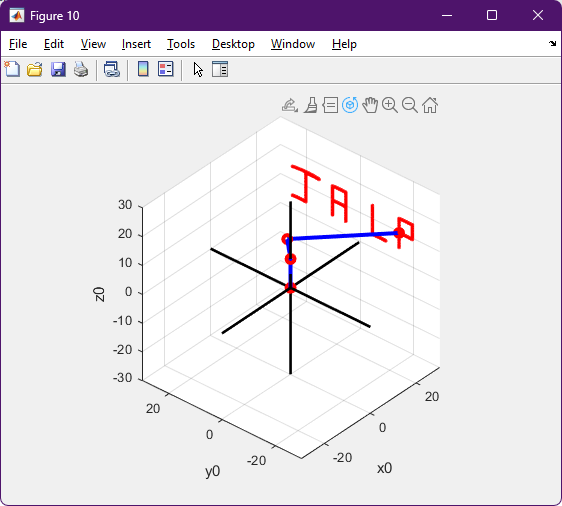
\includegraphics[width = 2.5in]{sim.png}
        \caption{Simulation of the manipulator}
        \label{fig:sim}
    \end{figure}

    \section{Conclusion}
    To sum up, this project help us to understand and apply direct and inverse 

%Bibliography------------------------------------------
    \pagebreak
    \printbibliography
%END---------------------------------------------------

%Appendix if required
    \pagebreak
    \appendix
    \section{Matlab code}
    Here is the code use for the simulation file on Matlab.
\% Jose Antonio Lara Perez\\
\% IRC 7B\\
\% WRITING OUR INITIAL WITH THE MANIPULATOR:\\
\%Variables for the Links
\\L2 = 10;
\%Vector of Desired Positions
\\Vx = [30 30 30 30 30 30 30 30 30 30 30 30 30 30 30 30 30 30 30];
\\Vy = [25 15 20 20 25 10 10 5 5 5 10 -5 -5 -10 -15 -15 -20 -20 -15];
\\Vz = [15 15 15 5 5 5 15 15 5 10 10 15 5 5 5 15 15 10 10];
\\Vdraw = [1 1 1 1 0 1 1 1 1 1 0 1 1 0 1 1 1 1 1];\\
\%Trayectories
\\tf = 5; \%Tiempo final para crear la trayectoria
\\t = 0;\\
\%Vector of Accumulated Trajectory\\
pAT = [];\\
\%Number of elements in vector of Desired Positions
\\Length\_ = length(Vx(1, :));
\\for j = 2 : Length\_\\
\% EXTERNAL DATA: POSITIONs TAKEN FROM POINTS of X \& Y\\
\%First Position
\\xi = Vx(j - 1);
\\yi = Vy(j - 1);
\\zi = Vz(j - 1);\\
\%Last position
\\xf = Vx(j);
\\yf = Vy(j);
\\zf = Vz(j);
\\
\% INVERSE KINEMATIC TO COMPUTE THE INTERNAL DATA: JOINT ANGLES: 10
\\
\%Calculus for trayectories

[d2i, d3i, t1\_i] = Inv\_Kin(L2, xi, yi, zi); %For the first point

[d2f, d3f, t1\_f] = Inv\_Kin(L2, xf, yf, zf); %for the last point

\%Coefficients for the first link
\\a10 = t1\_i;
\\a12 = 3\*(t1\_f - t1\_i)/(tf\^\ 2);
\\a13 = -2\*(t1\_f - t1\_i)/(tf\^\ 3);
\\
\%Coefficients for the second link
a20 = d2i;
\\a22 = 3\*(d2f - d2i)/(tf\^\ 2);
\\a23 = -2\*(d2f - d2i)/(tf\^\ 3);
\\
\%Coefficients for the third link
\\a30 = d3i;
\\a32 = 3\*(d3f - d3i)/(tf\^  2);
\\a33 = -2\*(d3f - d3i)/(tf\^\ 3);
\\
\\for t = 0:0.1:tf  
\%Trayectories
\\thT = a10 + a12\*t\^ 2 + a13\*t\^\ 3; 
\\d2T = a20 + a22\*t\^ 2 + a23\*t\^\ 3;
\\d3T = a30 + a32\*t\^ 2 + a33\*t\^\ 3;

[T01, T02, T02f, T03] = Dir\_Kin(thT, d2T, d3T, L2);


\% OBTAINING JOINT STRATEGIC POSITION VECTORS
\% TO DRAW THE MANIPULATOR
\\p0 = [0; 0; 0];
\\p1 = [T01(1, 4); T01(2, 4); T01(3, 4)];
\\p2 = [T02(1, 4); T02(2, 4); T02(3, 4)];
\\p2f = [T02f(1,4); T02f(2,4); T02f(3,4)];
\\p3 = [T03(1, 4); T03(2, 4); T03(3, 4)];
\\
\% CARTESIAN COORDINATE SYSTEM 3D:
\\figure(10);
\\clf(10);
\\view(3);
\\axis([-30, 30, -30, 30, -30, 30]);
\\
\\plot3([-30, 30], [0, 0], [0, 0],'-k', 'LineWidth',2); \% Axis x
\\hold on; grid;
\\xlabel('x0'); ylabel('y0'); zlabel('z0');
\\plot3([0, 0], [-30, 30], [0, 0],'-k', 'LineWidth',2); \% Axis y
\\plot3([0, 0], [0, 0], [-30, 30], '-k', 'LineWidth',2); \% Axis z
\\axis equal;
\% DRAWING THE MANIPULATOR
\% Links:
\\plot3([p0(1), p1(1)], [p0(2), p1(2)], [p0(3), p1(3)], '-b', 'LineWidth', 3);
\\plot3([p1(1), p2(1)], [p1(2), p2(2)], [p1(3), p2(3)], '-b', 'LineWidth', 3);
\\plot3([p2(1), p2f(1)], [p2(2), p2f(2)], [p2(3), p2f(3)], '-b', 'LineWidth', 3);
\\plot3([p2f(1), p3(1)], [p2f(2), p3(2)], [p2f(3), p3(3)], '-b', 'LineWidth', 3);
\\
\%Joints:
\\plot3([p0(1), p0(1)], [p0(2), p0(2)], [p0(3), p0(3)], '-or', 'LineWidth', 3);
\\plot3([p1(1), p1(1)], [p1(2), p1(2)], [p1(3), p1(3)], '-or', 'LineWidth', 3);
\\plot3([p2(1), p2(1)], [p2(2), p2(2)], [p2(3), p2(3)], '-or', 'LineWidth', 3);
\\plot3([p2f(1), p2f(1)], [p2f(2), p2f(2)], [p2f(3), p2f(3)], '-or', 'LineWidth', 3);
\\plot3([p3(1), p3(1)], [p3(2), p3(2)], [p3(3), p3(3)], '-or', 'LineWidth', 3);

    \%Storage all points reached by the tool for Drawing purposes  
    \\if Vdraw(j - 1) == 1
    \\    pAT = [pAT, p3];
    \\end
    \\if length(pAT) \~\ =0
    \\    plot3(pAT(1, :), pAT(2, :), pAT(3, :), '.r', 'LineWidth', 4);
    \\end % A delay to see the picture for a while.
\\end
\\end


    %Copy code and paste here

    \label{sec:matlabcode}
    


\end{document}